%% LaTeX_Thesis_Template.tex
% An unofficial LaTeX template for Cranfield theses.

%%
% This document is an example of the use of the unofficial "cranfieldthesis" 
% LaTeX style file.  I hope it's useful, and good like.

\documentclass[12pt]{book}

\usepackage[utf8]{inputenc}
% Use the custom "cranfieldthesis" LaTeX style file. 
\usepackage{cranfieldthesis}
\usepackage{xcolor}
\usepackage{graphicx}
\usepackage{float}
\usepackage{caption}
\usepackage{subcaption}

% By default, LaTeX uses a serif font - these are traditionally thought to be
% easier to read.   If you'd prefer sans-serif, please uncomment the 
% following line.
%\renewcommand{\familydefault}{\sfdefault}

\title{Development of Physics or HPC Optimisation of a parallel 2D lattice Boltzmann solver using GPUs/CUDA}
\author{José Oliveira}
\date{August 2017}
\school{Aerospace, Transport and Manufacturing}
\course{Computational \& Software Techniques In Engineering}
\degree{MSc}
\academicyear{2016--2017}
\supervisor{Dr Irene Moulitsas}
\copyrightyear{2017}


\begin{document}


%% Front matter
%
% This is where we do the title page, etc.
%

\frontmatter

% Standard-Form Title Pages
\maketitle

% Abstract and Keywords
\begin{abstract}
    Type your abstract here.
    \section*{Keywords}
    Keyword 1; keyword 2; keyword 3.
\end{abstract}

% Table of Contents
\sstableofcontents

% List of Figures
\sslistoffigures

% List of Tables
\sslistoftables

% The list of abbreviations can't be automatically generated so you need to populate it yourself
\begin{listofabbreviations}
    \abbrev{CUDA}{Compute Unified Device Architecture}
    \abbrev{CFD}{Computational Fluid Dynamics}
    \abbrev{GPGPU}{General-purpose computing on graphics processing units}
    \abbrev{GPU}{Graphics Processing Unit}
    \abbrev{LBM}{Lattice Boltzmann Method}
\end{listofabbreviations}

% Acknowledgements
\chapter{Acknowledgements}
The author would like to thank \dots

%% Main Matter
%
% This is where we include the main thesis content.
%
\mainmatter

\chapter{Introduction}

\chapter{Literature review}
In this chapter, we will be taken into the broad field of the Lattice Boltzmann method using the CUDA platform. The topic of this thesis is associated with a number of different study areas, such as Computational Fluid Dynamics, Lattice Boltzmann method, High performance computing and GPGPU. We will then present an extensive literature review on these themes in the remaining of this chapter. Firstly, we will look into Computational Fluid Dynamics and the most commonly used approaches to it. Then we will be giving an overview on the Lattice Boltzmann method. Afterwards we will discuss how it is possible to employ parallelisation techniques in scientific computing. Finally we will review some previous works in this area.
\section{Computational Fluid Dynamics}
Computational Fluid Dynamics (CFD) comes from the need to model fluid flows and associated processes.
A wide range of applications come from studying CFD, notably:
\begin{itemize}
\item Aircraft design \cite{aircraft_cfd}
\item Solid particle erosion \cite{partic_erosion_cfd}
\item Wind flow simulation \cite{wind_flow_cfd}
\item Combustion chamber simulations \cite{combust_cfd}
\item Environmental and weather prediction \cite{weather_pred}
\item Automotive and motor sports \cite{america_cup,race_car_wing}
\end{itemize}

CFD can be used as a design and troubleshooting tool, as well as making the process dynamics easier to understand. It is used extensively by scientists and researchers, but it also has innumerable applications in the industry. CFD simulations is a viable tool for manufacturing because it eliminates expensive simulations.\par
 As such, it is the science of determining a solution to fluid flow through space and time \cite{cfd_present}. The models needed to calculate the fluid computations include:
\begin{itemize}
\item	Flow geometry
\item	Differential (Governing) equations – These describe the physics and chemistry of the flow
\item Boundary and initial conditions
\item	Discretization of the domain
\end{itemize}



\subsection{Macroscopic scale}
In this approach, the fluid can be seen as a collection of a huge number of particles. To solve these governing equations, one needs to apply conservation of energy, mass and momentum \cite{lbm_springer}. But since these equations are difficult, or even impossible to solve analytically, discrete schemes, boundary and initial conditions are used to convert these equations into a system of algebraic equations. These equations can then be solved until an appropriate solution is produced. 
\par These problems are usually solved using Navier-Stokes equations that describe the fluid being solved as a continuum, which apply Newton's second law to fluid motion.

\subsection{Microscopic scale}
If we consider the fluid to be represented by individual particles then we will fall under the microscopic approach. In this approach, there is no definition of temperature or viscosity and collision between particles needs to be considered. Thus one needs to solve the differential equation of Newton’s second law \cite{lbm_springer}. Hence, the location and velocity of each particle needs to be taken into account.
	\par We can easily see that this approach becomes unfeasible for normal fluid sizes as the number of equations needed to be solved grows to the order of billions (consider that one mole of water contains more than $6 \times 10^{23}$ molecules.


\section{Lattice Boltzmann Method}
The Lattice Boltzmann method (LBM) is a mesoscopic scale approach to CFD and was first introduced as a Lattice-Gas Automata for the Navier-Stokes Equation \cite{gasautomata}. It is used to describe a fluid based on probabilities using the Maxwell-Boltzmann equation in the fluid’s equilibrium state \cite{lbm_springer}. 
\par In this method, we do not consider the individual characteristics of each particle. By grouping particles together in a D2Q9 (nodes containing 9 particles for 2D problems - Fig \ref{fig:d2q9})  or in a D3Q19 (nodes containing 19 particles for 3D problems - Fig \ref{fig:d3q19}) model, we can analyse the behaviour of the particles collectively  \cite{lbm_springer}. 

\begin{figure}[H]
\centering
  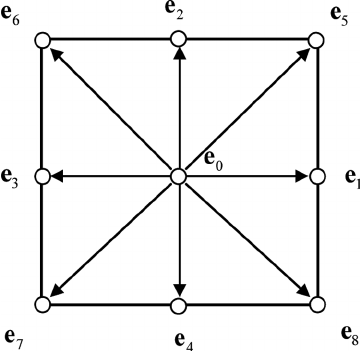
\includegraphics[width=0.3\linewidth]{Resources/Images/d2q9.png}
  \caption{2D LBM model using 9 particles. (D2Q9)}
  \label{fig:d2q9}
\end{figure}

\begin{figure}[H]
\centering
  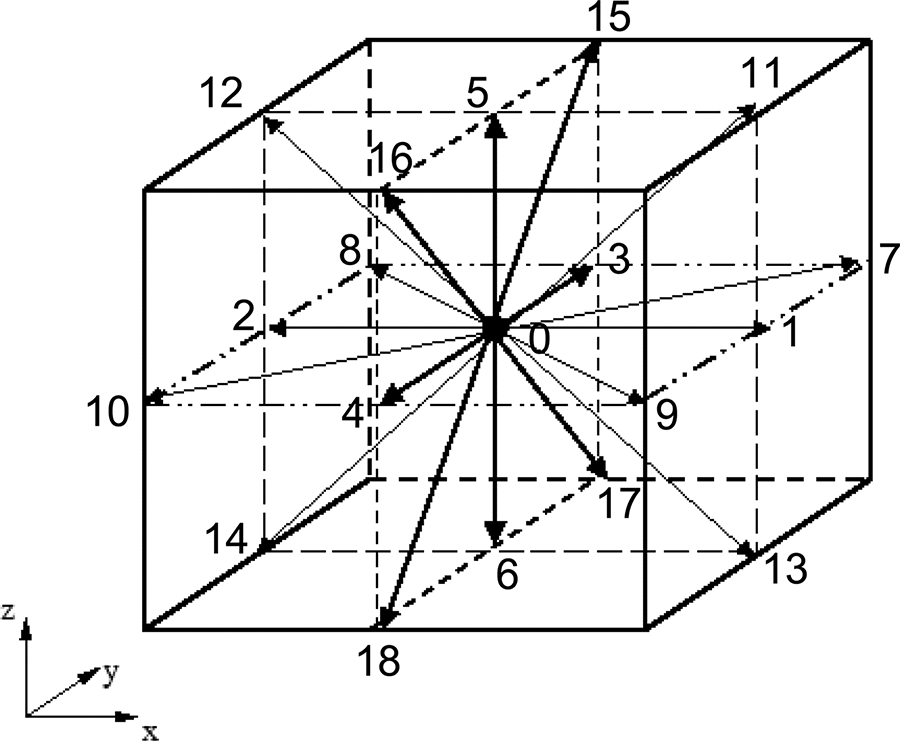
\includegraphics[width=0.3\linewidth]{Resources/Images/d3q19.png}
  \caption{3D LBM model using 19 particles. (D3Q19)}
  \label{fig:d3q19}
\end{figure}

\par
This way we can reap the advantages of both the macro and microscale approaches without the need of high end computers \cite{lbm_springer}. Since communications between nodes are very limited, LBM also offers the possibility of employing parallel computing to achieve the solution in even faster times.

\subsection{Multiphase flow}
Multiphase flows represent the simultaneous flow of materials in different states (phases). As such, multiphase flows have an enormous spectrum of representation and stand for interactions between gas/solid flows, liquid/solid flows or even liquid/liquid flows with different chemical properties \cite{multiphase}.\par
These simulations present challenging problems because of inherent difficulties during modelling and the importance of engineering applications. However, the Lattice Boltzmann method provides an alternative for these simulations due to it's relative simplicity when compared with traditional Navier-Stokes equation \cite{chenDoolenMP}.
\par These flows have several applications in the scientific and industrial community, ranging from pourous media fluid interactions \cite{pourous} to flows containing gas bubbles dispersed in liquids \cite{gasBubble}. Furthermore, almost every processing technology must take multiphase flows into account, including cavitating pumps, papermaking and many others \cite{multiphase}.
\par Several implementation strategies exist for Multiphase flows, however, for the purpose of this thesis, we will first follow the simple ''two-color'' approach first proposed by Gunstensen et al \cite{gunstensen}.


\section{High Performance Computing}
As humanity evolves, so too does our desire for expanding previous unobtainable goals. As computer technology kept progressing further and further, we soon realised that some problems simply took too many resources to be completed.\par
Figure \ref{fig:moore} shows the evolution of computing power over the past 120 years. Moore's Law states that ''processor speeds, or overall processing power for computers will double every two years'' \cite{moore}. Note that the last 7 most recent data points are NVIDIA GPUs.

\begin{figure}[H]
\centering
  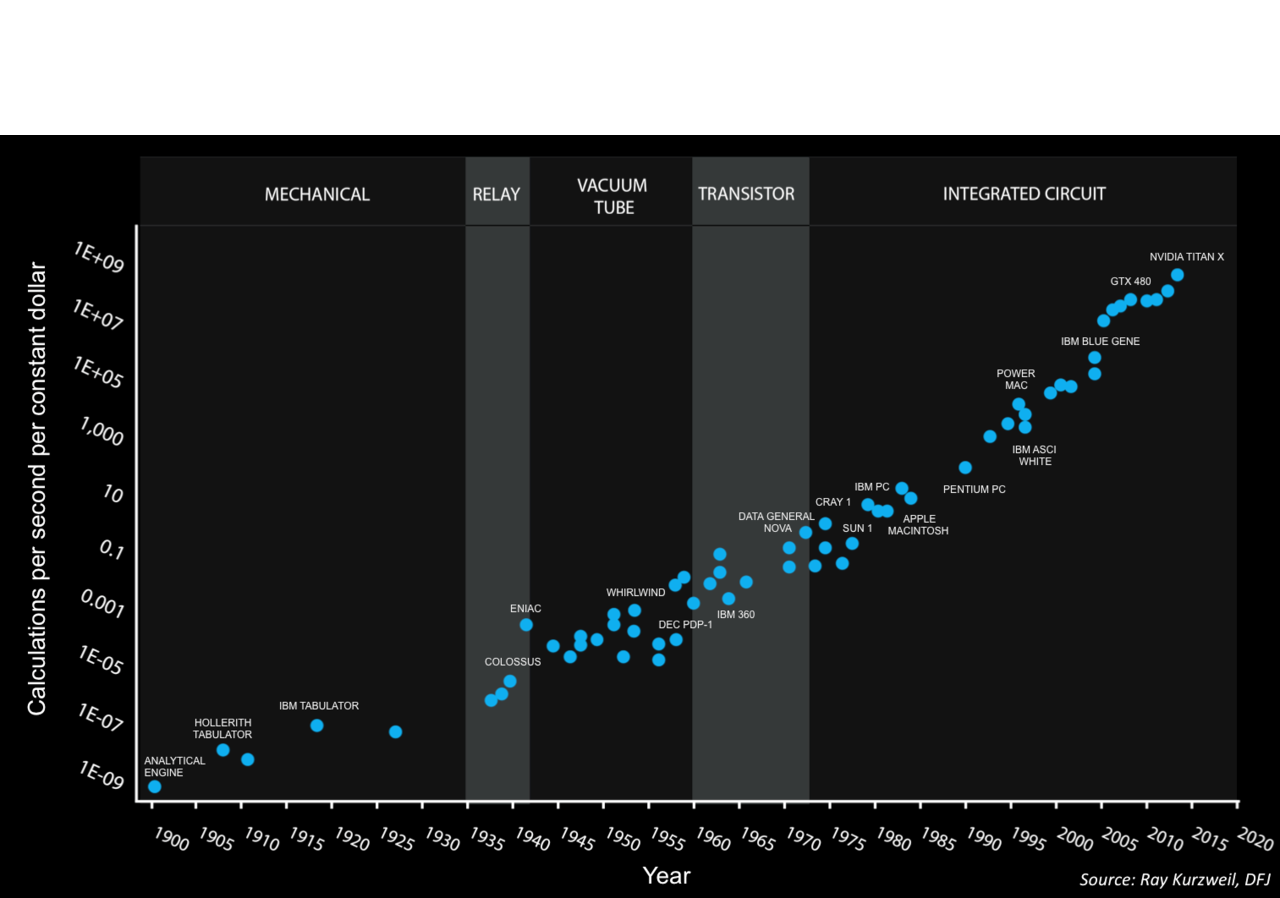
\includegraphics[width=0.6\linewidth]{Resources/Images/moore120.png}
  \caption{Moore's law over 120 years}
  \label{fig:moore}
\end{figure}

However, this evolution in computational power could only be achieved by combining CPU cores together.
So what if we focused our efforts in splitting the workload, effectively using the multiple cores available to produce a solution?\par
High performance computing (HPC) comes from the harnessing of computer power to deliver a much higher performance that one could not obtain from a typical computer. To this end, we can talk of HPC as being a collection of computer resources, all of them working simultaneously to achieve a solution of the same problem. Problems that could otherwise take weeks, months or even years can now be solved in minutes, hours or days under these powerful devices. However, different parallelisation strategies for splitting the workload emerge, depending on the underlying hardware. \par
It is also important to understand that parallel computing is achieved with the help of processors that will execute different calculations or processes simultaneously. To measure the parallelisation's efficiency, it is worth introducing the term Speed-up. The Speed-up is the ratio of the execution time of the parallel algorithm on a single processor with the execution time of the parallel algorithm on P processors \cite{irenehpc}. However, Amdahl's law states that ''in parallelization, if P is the proportion of a system or program that can be made parallel (...), then the maximum speed-up that can be achieved using N number of processors is $\frac{1}{\left(1-P\right)+\frac{P}{N}}$'' \cite{amdahl}. This means that our parallelisation efforts are limited by the amount of work that can be parallelised and, theoretically, should follow the distribution represented in Figure \ref{fig:amdahl}. 

\begin{figure}[H]
\centering
  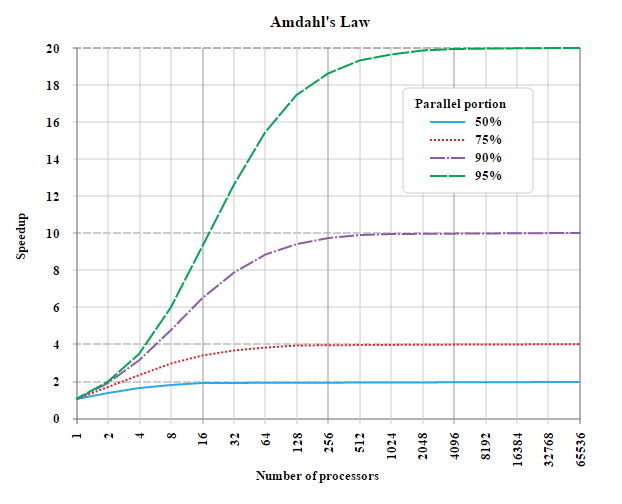
\includegraphics[width=0.6\linewidth]{Resources/Images/amdahl.png}
  \caption{A graphical representation of Amdahl's law}
  \label{fig:amdahl}
\end{figure}

\subsection{Distributed memory}
Following a distributed memory architecture for parallel computing means that each processor will have it's own independent local memory. In these systems, all the work that one process executes remains local to it, without interfering with the address space of all other processors. Hence, to solve meaningful computations, a communication network needs to be established in order for processes to share data with each other. Such is the case of the Message Passing Interface (MPI).\par
This means that this architecture is very scalable: with each processor being added to the system the size of the total memory increases. Also, each processor will be able to access it's own memory rapidly and without interference, reducing the usual constraint of memory access penalties.
\par However, this type of system requires a higher degree of skill from the programmer. The programmer will be the one responsible for most of the details of memory passing between processors and will need to ensure that no race conditions or deadlocks arise from the data communication. Also, whenever data from another processor is needed, the latency of the bandwidth in the network will introduce a heavy time penalty to the computations, as this data will need to be communicated before computations can be performed over it.
\subsection{Shared memory}
In a shared memory architecture, each processor is able to access all memory as global address space. This means that data can be handled seamlessly between processors, making programs easy to read and easy to write. An example of this model can be the Open Multi-Processing (OpenMP) API, which supports shared memory multiprocessing programming in C, C++ and Fortran. In this architecture, processors can operate independently while having access to the same memory resource pool as all other processors. Therefore, changes in the data handled by one process is visible and updated for all others. \par
This means that the programmer can have a user-friendly environment while working on his/her algorithm. All details concerning data flow between processes are abstracted, making this model very beneficial for users with little to no background in parallel programming. Also, the data being shared between processors is fast and uniform, making the penalties of memory access of this shared data less penalizing than in the distributed memory model.
\par However, this architecture presents little memory scalability, since adding more CPUs will increase the traffic of the shared memory path. Also, the programmer will have to pay close attention to memory access so as to prevent memory violation and ensure a correct synchronization of the access to the global adress space.

\subsection{GPGPU}

General Purpose computing on Graphical Processing Units stands for the use of Graphics Processing unit (GPU) to perform computations on applications normally performed by the CPU. One of the main advantages of using this approach is the amount of cores that a single GPU has. While a typical desktop CPU has up to 4 cores, a GPU can have thousands of cores, allowing users to take advantage of its massively parallel architecture. GPUs can now solve problems that were traditionally solved by the CPU. This is a big improvement, since GPUs are cheaper to acquire and more powerful than CPUs.\par
	NVIDIA then developed CUDA. CUDA code allows programmers to take advantage of GPUs by employing a unified shader pipeline under the familiar C language \cite{cuda_by_example}. Users were no longer required to have specific knowledge of OpenGL or DirectX and could now perform general computations (rather than graphic-specific computations) whilst benefiting from the massive computational powered offered by GPUs. 
	\par Programmers could now use the macros defined by CUDA to harness the full power of the GPU with a relatively small learning curve. If the user is already familiar with C language, then he can pick up on the details of the framework quickly. While this may seem like a big improvement, almost nothing comes without some disadvantages. CUDA can be excessively complicated to those unfamiliar with parallel programming. Although it offers the possibility of competing with several CPUs linked together, to optimise the kernel calls (device specific functions) takes a big attention to details and some knowledge on how the underlying hardware works. Users should not take this approach light-heartedly as they can easily become encumbered with work when compared to a simpler to use framework (such as OpenMP).  

\section{Previous parallelisation works}
This thesis is a continuation of work that started some years ago in Cranfield University. As such, the work from the previous students needs to be analysed. \par
In 2014, Tamás Józsa and Máté Szőke, adapted two different in-house C and C++ codes into one single C code unifying the advantages of each one of the two original codes \cite{jozsa_thesis,szoke_thesis}. Józsa then parallelised the critical parts of the C code using CUDA and ran tests on the Fermi GPU Cluster from Cranfield, achieving a three times speed-up in general, with a peak of 15 times speed-up \cite{jozsa_thesis}. \par
Szőke proposes a CPU parallelisation approach using Unified Parallel C, which is a Partitioned Global Address Space language\cite{szoke_thesis}. This means that it is possible to use shared memory to compute the solution. However, the author verified that a local memory-based approach (like MPI) provided the best results. He also compared the results obtained with the ones obtained by Józsa on the CUDA approach. They found that to achieve the same speed-up as that of a single GPU card, one needs an entire workstation (16 threads in the case of Astral) \cite{szoke_thesis}.\par
In 2015, Ádám Koleszár continued the work and further optimised the parallel version of the LBM method using CUDA \cite{koleszar_thesis}. He did an excellent job, resulting in a 10 times faster execution than the previous 2D parallel solver, which means that his new optimised code was 30 times faster than the original, in-house, serial solver.\par
Finally, in 2016, Maciej Kubat proposed a new version of the LBM solver.Firstly he converts the 2D parallel solver to a 3D parallel solver which entailed a major re-engineering of the code, from data containers to logic cycles \cite{maciej_thesis}. After first trying for a direct adaptation, he found that his code was too slow to produce meaningful solutions. After optimising his own code he was able to reach an almost one hundred times speed-up.
However, Kubat states that a lot can be done to improve his code, from boundary conditions to code readability and maintainability. 
\chapter{Methodology}
\section{In-house LBM solver}
The implementation of a 3D multiphase flow using the Lattice Botzmann method will be based on an existing in-house code. As such, the first step in developing the new solver is to acquire a good understanding of how the previous solver works, specifically, it’s structure and organisation, it’s input and output data, it’s performance and it’s depending software (if any). Furthermore, the previous code needs to be validated so as to provide and accurate foundation for the project being developed. Without this validation, it would prove to be an arduous work to discover whether the new solver is behaving correctly.
\subsection{Code organisation}
After spending some time analysing the LBM solver and debugging some of the core features, I was able to obtain a generous understanding of how the existing code is organised and where most of the necessary algorithms are located. The solver itself was very well documented and most of the solver’s features were written in a very user-friendly way. Because of this good work from the authors of this solver, the following flow chart, Figure \ref{fig:codeFlow}, was able to be made in a relatively small amount of time, which helps to gain a general understanding of the solver.

\begin{figure}[H]
\centering
  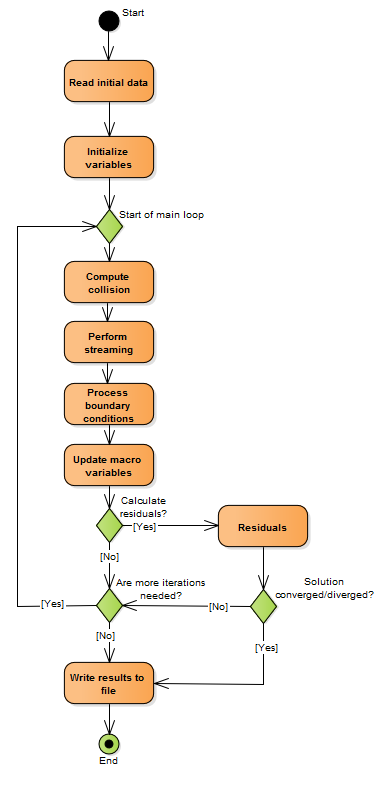
\includegraphics[width=0.5\linewidth]{Resources/Images/CodeFlowchart.png}
  \caption{A simplified flowchart of the solver's activity}
  \label{fig:codeFlow}
\end{figure}

The previous authors strived for a optimized and easy to use code. As such, the SetUpData.ini file contains all the information needed to build the problem to be solved. This file, combined with the mesh files that the user wishes to simulate, provide the initial step in running the solver. Note that external calculations need to be used to guarantee some aspects of the initial conditions, such as the Reynolds number.\par
Similarly, when the solver finishes computations, a Results folder is created containing information pertinent to the solution of the solver. These files include the final solution, the residuals, the run time, etc. The user also has the option of selecting which output format to produce the solution in (.vti, .dat or .csv).

\subsection{Performance}
This thesis will be based on the work of previous Cranfield MSc students. As such, the received solver needs to be validated regarding the established performance in Kubat’s thesis \cite{maciej_thesis}. To this end, I generated the same meshes as the ones used in his thesis, specifically the lid driven cavity 128 and 256. \par
The lid driven cavity is a commonly used benchmark test for CFD solvers. It consists of a cube with a moving lid on the top which acts as the inlet for the flows. The numbers refer to the number of nodes in each direction, i.e. cavity 128 represents a 128x128x128 cube, resulting in 2097152 nodes.
\par
The final run-times of both meshes were very similar to the ones previously obtained, as shown in Figure \ref{fig:compareTimes}. Because of this, we can be sure that our version of the solver is the same as the final one used by the previous authors during their theses. \par

\begin{figure}[H]
\centering
  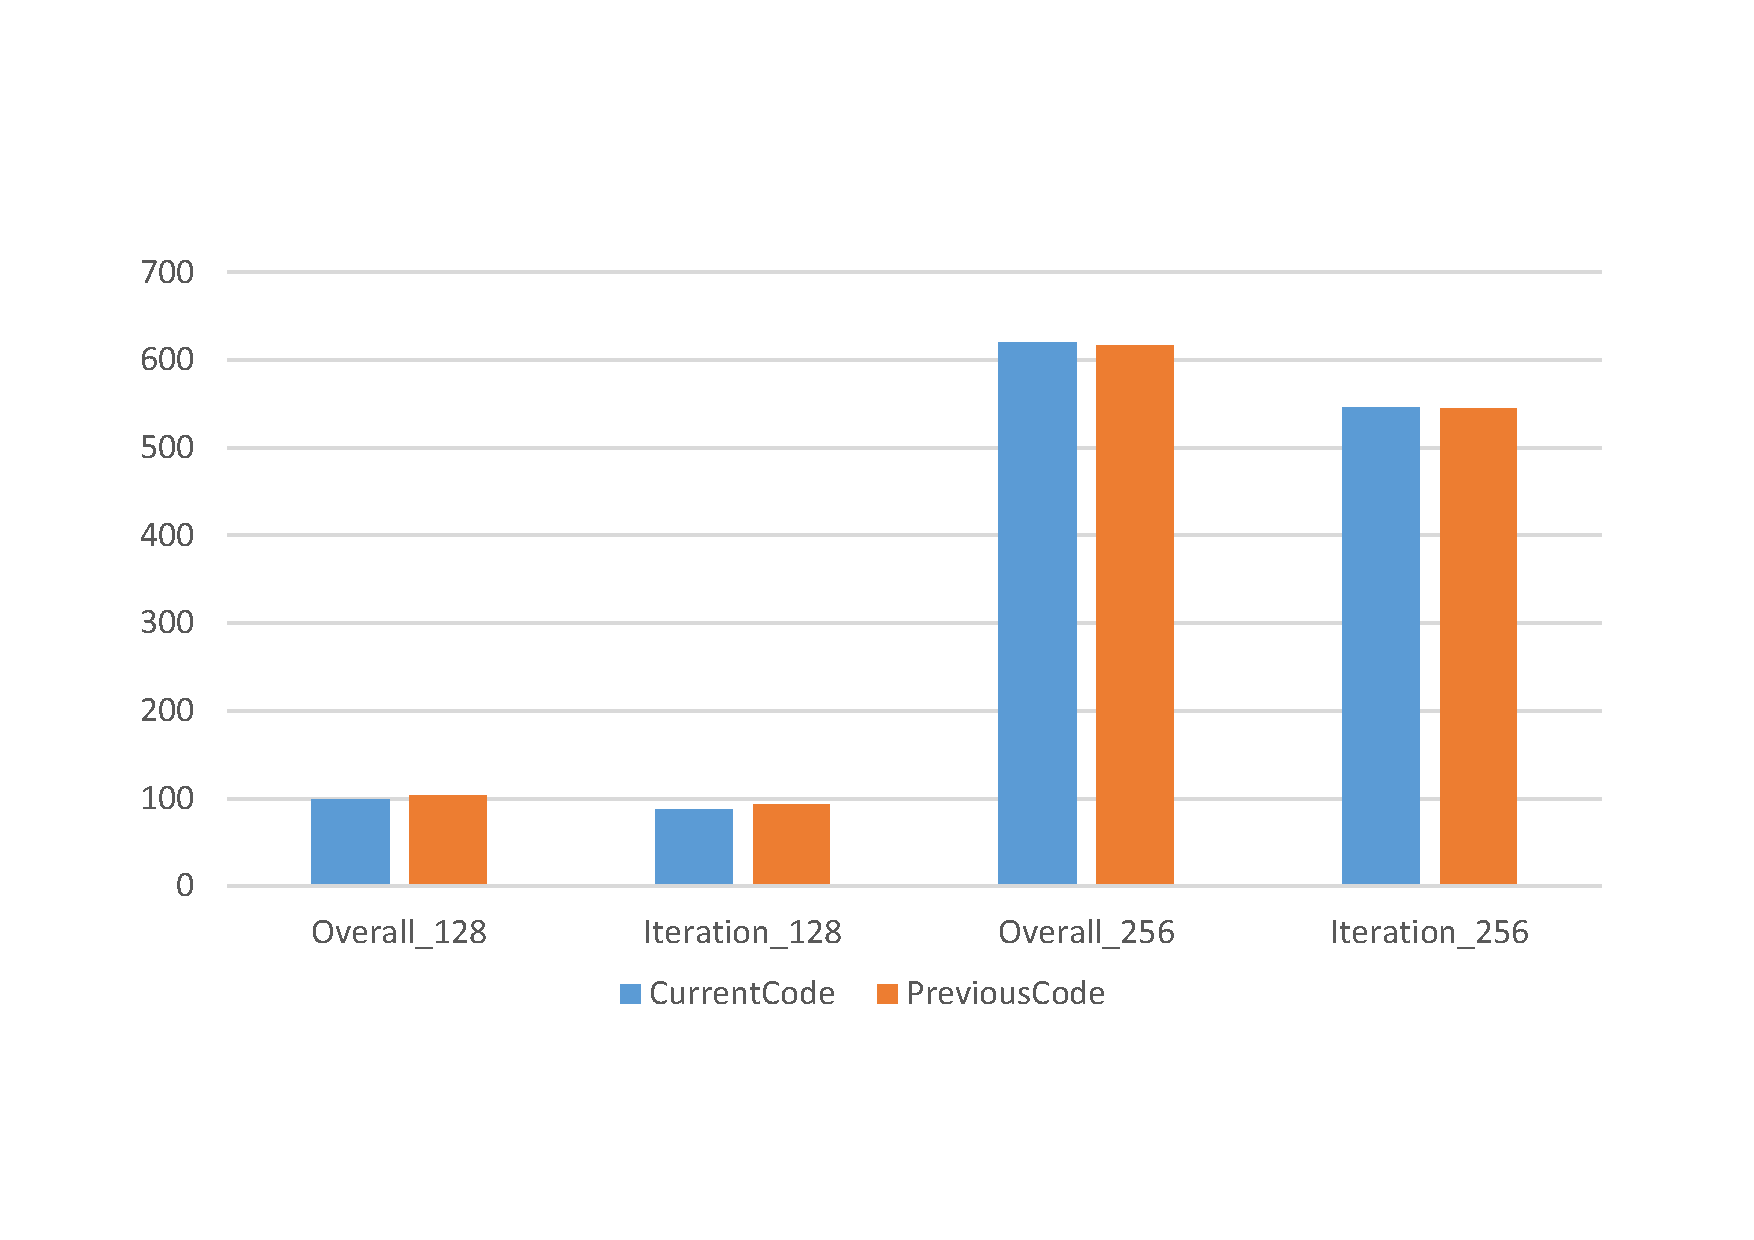
\includegraphics[width=0.9\linewidth]{Resources/Images/compareTimes.pdf}
  \caption{Runtime for Cavity\_128 and Cavity\_256}
  \label{fig:compareTimes}
\end{figure}


To gain a better understanding of the code, the solver’s run-times were profiled according to the main phases of the method. Figure \ref{fig:initialProfiling} shows that the solver spends about 40\% of it’s time calculating residuals. The residuals are used to check whether the solution has converged or diverged, making them a valuable method for potentially saving computation time (which in HPC centres means saving money). However, if the user is sure that the problem being solved needs to run for the specified iterations, he might be able to speed up the solver by not calculating the residuals, or even by specifying an interval of iterations before calculating residuals again.

\begin{figure}[H]
\centering
  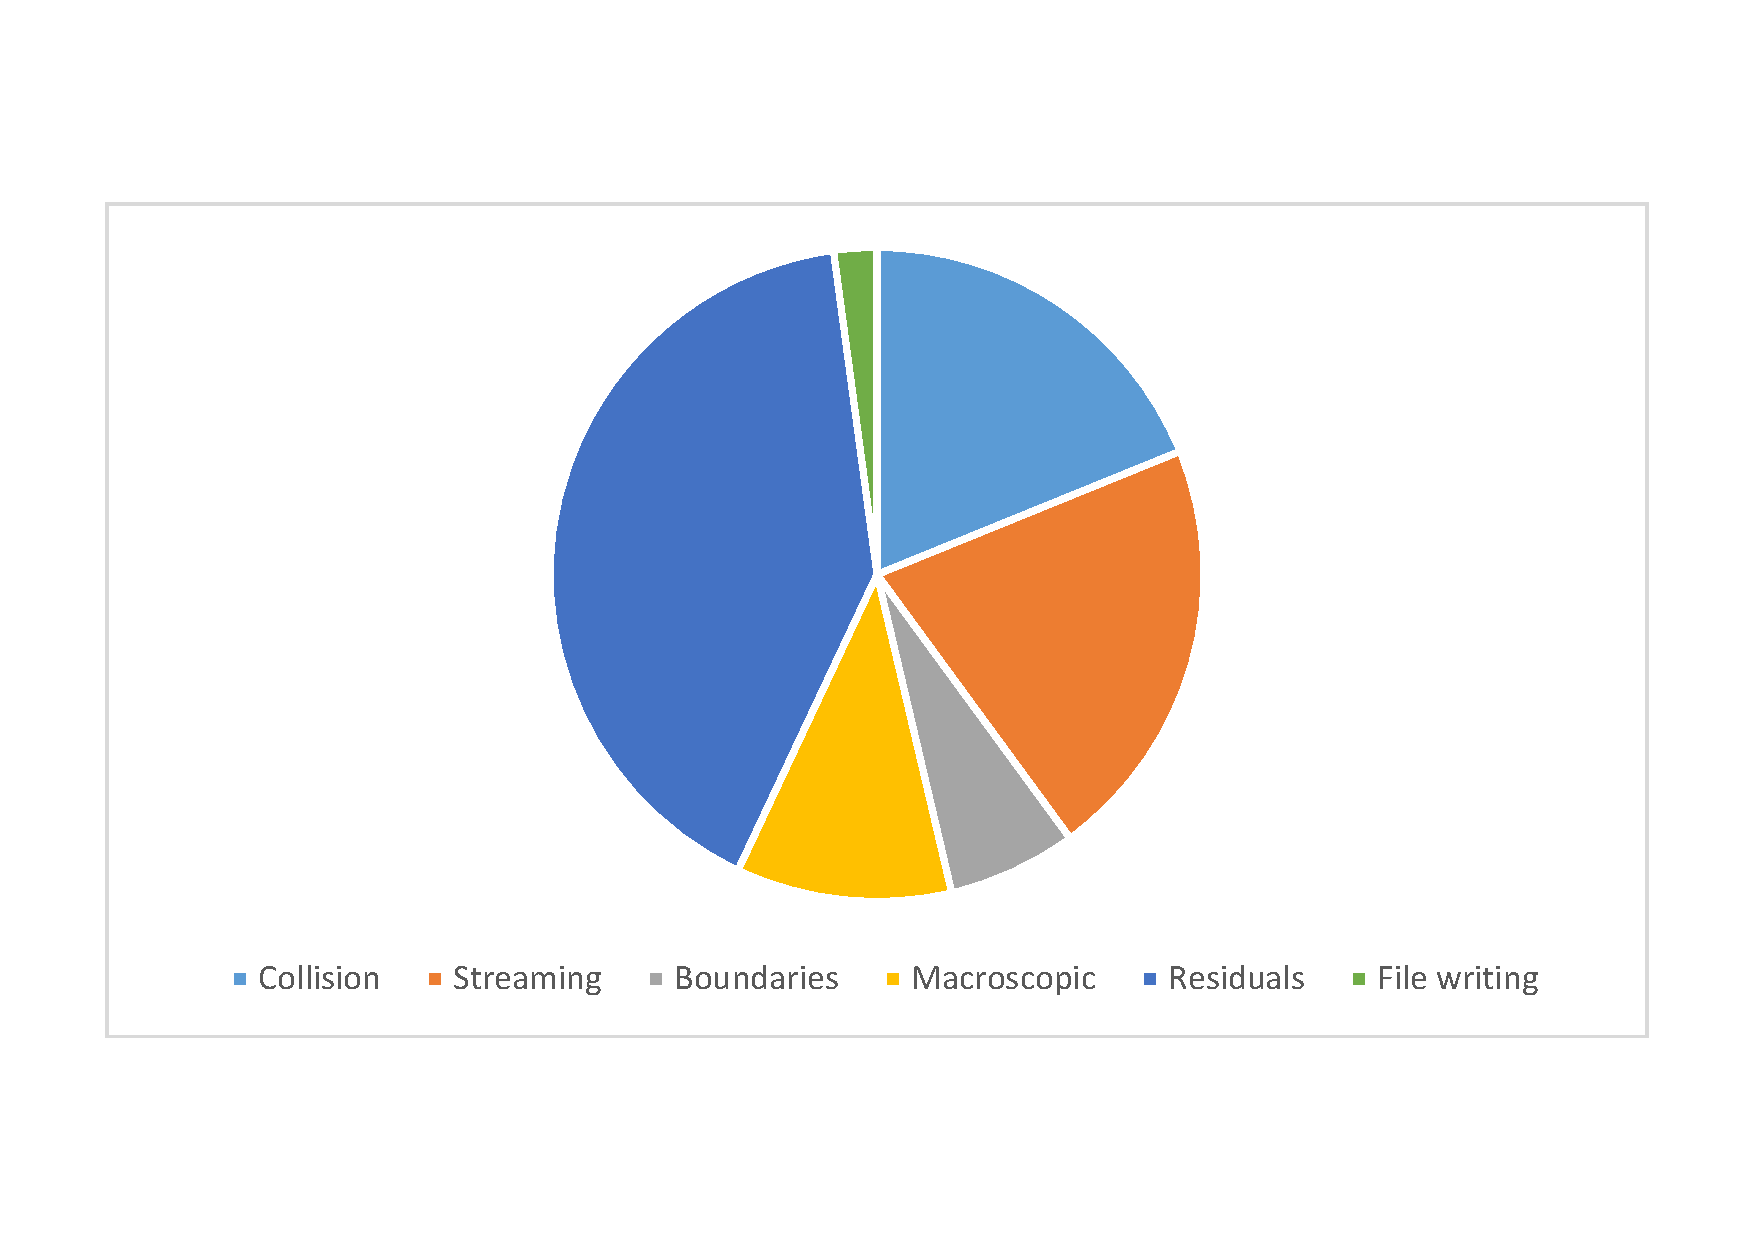
\includegraphics[width=0.9\linewidth]{Resources/Images/initialProfiling.pdf}
  \caption{Code profiling for the run-times of Cavity\_128 with MacroDiff residuals}
  \label{fig:initialProfiling}
\end{figure}

\par The remaining time is split between the collision, streaming and macroscopic values calculation, with boundary condition calculations and file writing occupying a less important slice of execution time. With this profiling, we now know which are the most critical parts of the software (residuals, collision and streaming) and can focus our efforts in optimising those areas when developing the method for multiphase flows.
\par Finally, the received solver was programmed to run with a 2D configuration in the kernel calls. Both the blocks per grid and threads per block are set up to run with an equal number of elements in the two directions. \textcolor{red}{The number of blocks is calculated dynamically with problem size in mind and sets 1 block per node.} However, the number of threads per block is declared statically with a value of 16x16. This means that the solver will use 16 threads in the x direction and another 16 in the y direction per block, meaning that each block uses 256 threads. To understand how this value affects the solver, I have benchmarked the solver using two more configurations for the Cavity\_128 and Cavity\_256 meshes.

\begin{figure}[H]
  \centering
  \begin{subfigure}{.49\textwidth}
  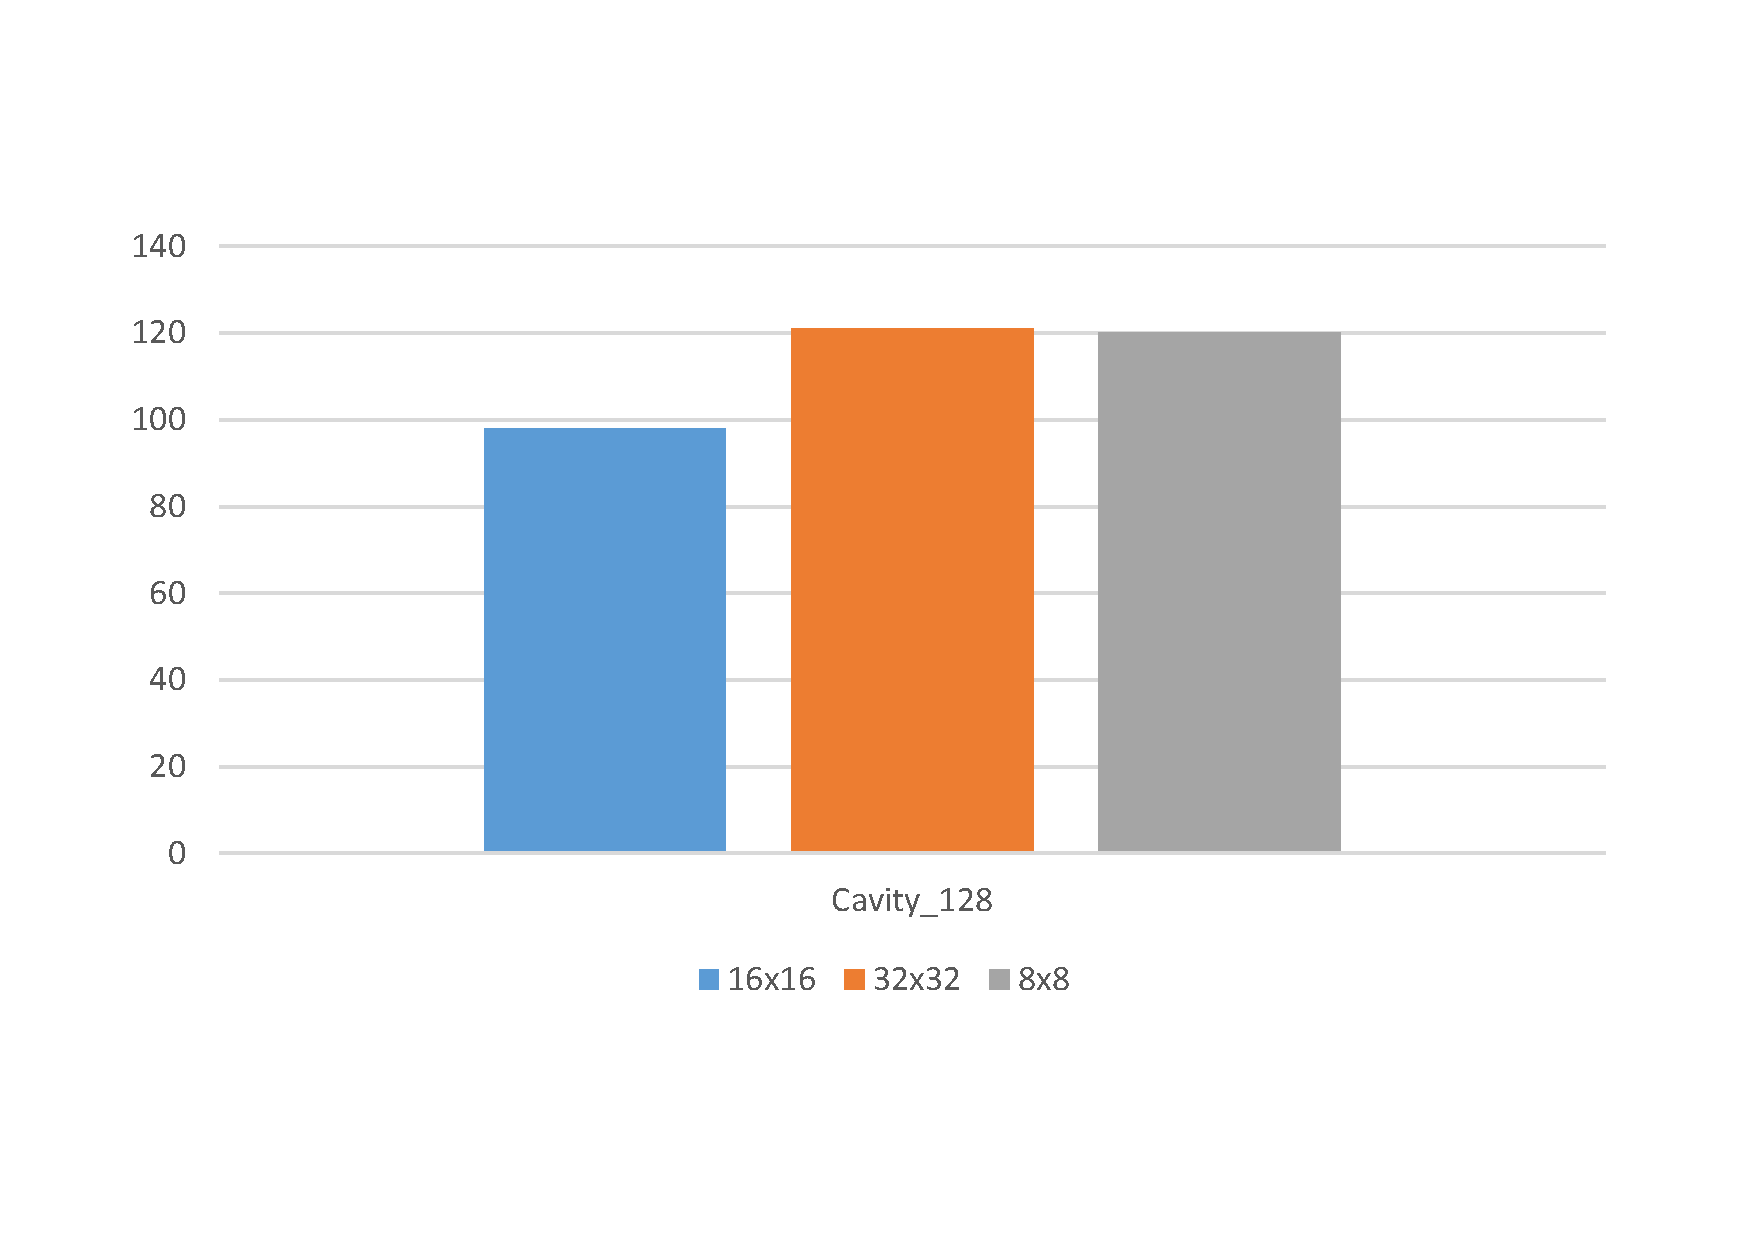
\includegraphics[width=\linewidth]{Resources/Images/timesThreads128.pdf}
  \caption{Cavity\_128}
  \end{subfigure}
  \begin{subfigure}{.49\textwidth}
  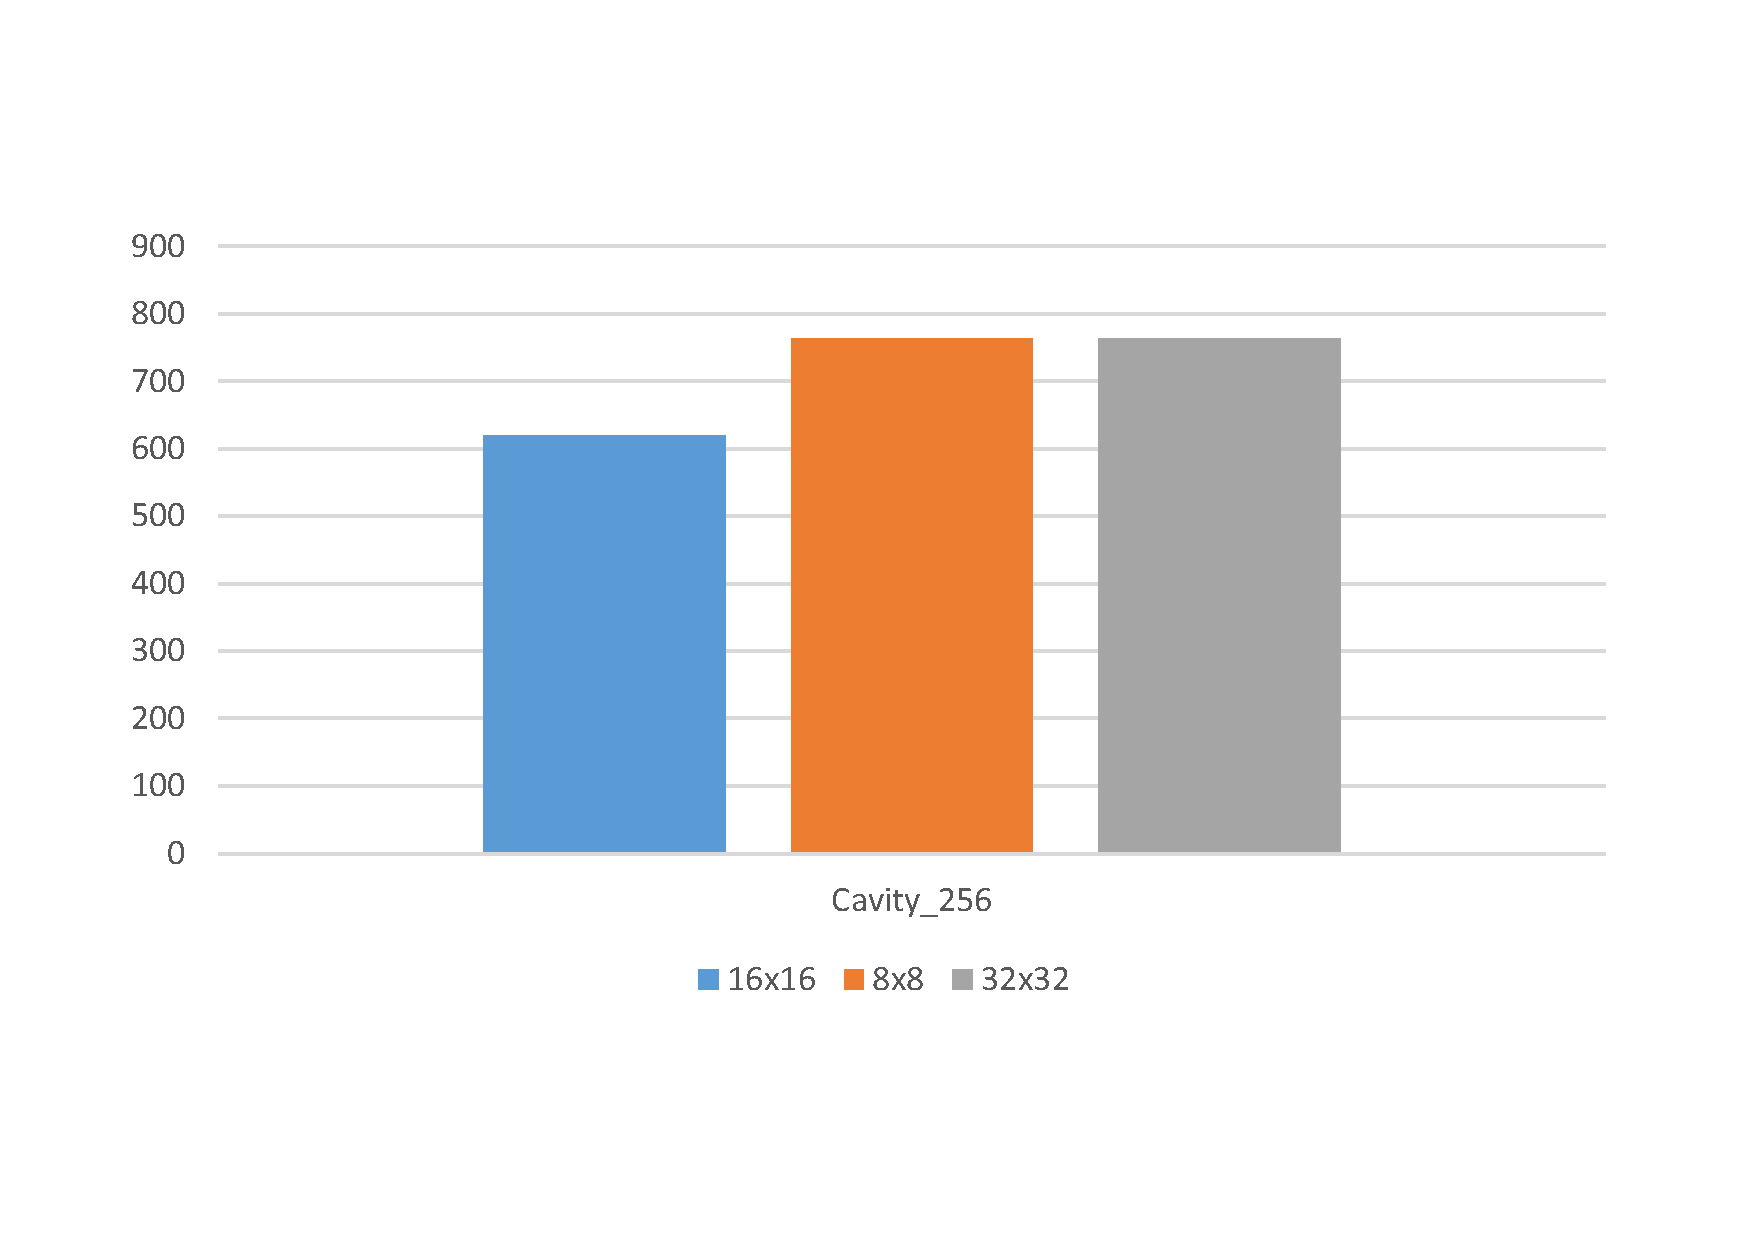
\includegraphics[width=\linewidth]{Resources/Images/timesThreads256.pdf}
  \caption{Cavity\_256}
  \end{subfigure} 
   \caption{Overall time comparison using three different threads per block configuration}
  \label{fig:timesThreads}
  \end{figure} 
  
  Figure \ref{fig:timesThreads} shows that the initial configuration (16x16) provides the best results. Because of this, the parallelisation strategy for the multiphase algorithm development will also start with this number of threads per block.


\subsection{Validation}
Now that the received code has been validated to perform under the same conditions as the final version used by the previous authors, we now have to verify whether the results that the received version is producing are the same as the final one. The validation of the results obtained throughout this project will be under the responsibility of Antonio González. As such, the details for this initial validation can be found in his thesis \cite{antonioThesis}.
\par This initial validation is essential for the development of a multiphase flow using the in-house solver. Without it, there would be no way of telling whether the solver would be functioning incorrectly due to a faulty algorithm implemented by us or if the solver was already producing wrong results. By doing so we can be sure that our code behaves correctly and that a proper result is achieved.


\chapter{Results and Discussion}
\chapter{Conclusions}

%% Back matter
%
% This is where we include appendices and references

\appendix

\bibliography{AllBib}{}
\bibliographystyle{plain}
\end{document}